\documentclass[aspectratio=169, xcolor=table]{beamer}

% fontenc rimosso: con XeLaTeX e fourier-otf non serve e può dare fastidio
\usepackage{fourier-otf} 
\usepackage{hyperref}
\usepackage{latexsym,amsmath,multicol,booktabs,calligra}
\usepackage{colortbl}      % robustezza con linee verticali/orizzontali
\usepackage{graphicx,listings,stackengine}
\usepackage{lipsum}
\usepackage{eurosym}
\usepackage{ragged2e}
\usepackage{etoolbox}
\usepackage{tikz}
\usepackage{pgffor}
\usepackage{natbib}

% --- IMPOSTAZIONI DEL TEMPLATE VERDE (TOR VERGATA) ---
\useoutertheme{miniframes}
\useoutertheme{infolines}
\setbeamertemplate{navigation symbols}{}

% Definizione del colore Pantone 7732 CP (Tor Vergata)
\definecolor{torvergata}{RGB}{0,122,51}

% Applicazione del colore agli elementi del tema
\setbeamercolor{palette primary}{bg=torvergata,fg=white}
\setbeamercolor{palette secondary}{bg=torvergata!90!black,fg=white}
\setbeamercolor{palette tertiary}{bg=torvergata!70!black,fg=white}
\setbeamercolor{palette quaternary}{bg=torvergata!50!black,fg=white}
\setbeamercolor{structure}{fg=torvergata} % Colora i titoli delle sezioni e i bullet point
\setbeamercolor{title}{fg=torvergata}
\setbeamercolor{frametitle}{fg=torvergata}
% ------------------------------------------------------

\author[Donato Pierno]{
    Nicola Milella\textsuperscript{2}, 
    Stefano Papa\textsuperscript{1, 2}, 
    \textbf{Donato Pierno}\textsuperscript{1, 2}, 
    James Tremewan\textsuperscript{3}
}

\title[From Words to Coalitions]{From Words to Coalitions: Communication in a Bargaining Game with\\ LLM Text Analysis.}
\subtitle{}
\institute{
    %\textsuperscript{1}University of Bari Aldo Moro, Bari, Italy\\
    \textsuperscript{1}Tor Vergata University of Rome, Italy\\ 
    \textsuperscript{2}CIMEO, Sapienza University of Rome, Italy \\ 
    \textsuperscript{3}HSE University, Moscow, Russia
}
\date[September, 3, 2026]{\small ESA, Barcelona, September 3\textsuperscript{rd}, 2026}

% defs
\def\cmd#1{\texttt{\color{red}\footnotesize $\backslash$#1}}
\def\env#1{\texttt{\color{blue}\footnotesize #1}}
\definecolor{deepblue}{rgb}{0,0,0.5}
\definecolor{deepred}{RGB}{153,0,0}
\definecolor{deepgreen}{rgb}{0,0.5,0}
\definecolor{halfgray}{gray}{0.55}

\lstset{
    basicstyle=\ttfamily\small,
    keywordstyle=\bfseries\color{deepblue},
    emphstyle=\ttfamily\color{deepred},    % Custom highlighting style
    stringstyle=\color{deepgreen},
    numbers=left,
    numberstyle=\small\color{halfgray},
    rulesepcolor=\color{red!20!green!20!blue!20},
    frame=shadowbox,
}

\begin{document}

\begin{frame}
    \titlepage
    \vspace*{-0.6cm}
    \begin{figure}
        \centering
        
\includegraphics[width=0.10\linewidth]{pic/LOGO - ATENEO_PANTONE 7732 CP_Variante1_20230307.png}
    \end{figure}
\end{frame}

\begin{frame}   
\tableofcontents[sectionstyle=show,
subsectionstyle=show/shaded/hide,
subsubsectionstyle=show/shaded/hide]
\end{frame}

\section{Motivation}

\begin{frame}{Motivation}\justifying
In many \textbf{decision-making bodies} (i.e., legislatures, city councils, school boards, and academic commissions), \textbf{decisions are reached after} extended negotiations, with \textbf{private meetings preceding public debate}. In rare cases, it is unrealistic to prevent confidential communications. 

 \vspace{0.5\baselineskip} 
 
\textbf{These meetings} are often criticized for promoting the formation of majority coalitions and, thus, undermining prosocial attitudes and outcomes.
\end{frame}

\begin{frame}{Research Questions}\justifying
We study how\textbf{ communication} protocols and the \textbf{distribution of payoffs} within a coalition \textbf{affect coalition formation} in a one-shot, three-player coalition game. 

\vspace{0.5\baselineskip}
\begin{itemize}
    \item Do messages differ between different communication protocols?
    \item Do aspects of communication  differ between communication protocols in the way they predict Persuasion to form coalitions?
    \item What individual characteristics predict Persuasion to form coalitions? And they differ between communication protocols?
    \item Choice–signal consistency they differ between communication protocols?
\end{itemize}
\end{frame}



\begin{frame}{Novelty}\justifying
    Our experiment provides insights into the frequent claims about \textbf{public and private communication in coalition formation}. This phenomenon is observed in a one-shot \textbf{bargaining game} (\citealt{TREMEWAN201633}).\footnote{Unstructured version of the well known \cite{baron1989bargaining} game.}
    
    \vspace{0.5\baselineskip}    
    We study, under private communication, the effect of heterogeneous \textbf{payoffs distribution} within  coalition how change the way participants persuade each other.
    
    \vspace{0.5\baselineskip}    
    Finally, we extract Topic from communication, through \textbf{TopicGPT}(\citealt{pham2024topicgpt, fieberg2025predicting}).
\end{frame}
%``
\section{Experimental Design}

\begin{frame}{Experimental Design}\justifying
     \begin{itemize}
     \item Online experiment between subjects with 1443  prolific participants, lasting 15 min, average payment \$6.50.\\
     \textbf{Groups by treatment}: Baseline N= 160, Public N= 158, Slacker N= 163.
     \vspace{0.5\baselineskip}  
    \item Experimental flow:
    \begin{itemize}
        \item Bargaining game with free form two-sided communication;
        \item Individual characteristics;
    \end{itemize}    
\end{itemize}
\end{frame}
\begin{frame}{Experimental Design: Bargaining Game}\justifying
    This part consists in dividing an exogenous surplus within a triad. The division occurs through three options. An option that receives at least two votes is implemented for the real payment.
    
    \vspace{0.5\baselineskip} 
    \textbf{Options:}
    \vspace{0.2\baselineskip} 
    \begin{itemize}
        \item Two-way split with only one other participant (i.e., 3,3,0);
        \item Three-way split among all participants (i.e., (2,2,2), \textbf{\textit{equal}} allocation).
        \item Each subject is assigned a \textbf{fictitious identity} with a unique color label (i.e., Red, Blue or Green), and matched in a group of three(triad);
    \end{itemize}
    \vspace{0.5\baselineskip} 
    During the \textit{$1^{st}$} part, participants can send messages through our communication environment.
\end{frame}


\begin{frame}{Experimental Part One: Bargaining Game}\justifying
\renewcommand{\footnotesize}{\scriptsize} 
    We employ an unstructured\footnote{Recent uses of unstructured bargaining games: \cite{tremewan2018voting}; \cite{baranski2024experiment}; \cite{kamm2024commitment}} one-shot bargaining game with communication. Participants are randomly matched in a triad after correctly answering the CQs.\\
    \vspace{0.5\baselineskip}  
    After the free-form communication and before their final decision, each participant is required to send a pre-written message (\textbf{Intentions}) to each of the other two participants.
    
    \vspace{0.5\baselineskip}
    Intentions:
    \begin{itemize}
\item I wish to split the payoff equally with Participant Green.
\item I wish to split the payoff equally with Participant Red.
\item I wish to split the payoff equally with both of the other participants.
\end{itemize}
    \vspace{0.4\baselineskip}
    \textbf{No majority} (i.e., each chooses a different option): the group fails to coordinate, and the disagreement payoff is \$0 for the triad.
\end{frame}




\begin{frame}{Treatments}\justifying
\label{treatments}
\textbf{Communication:}
\begin{itemize}
    \item \textit{Public} (baseline): each participant in the baseline group can \textbf{read the messages in which they are not directly involved}. After the communication, they are able to read all the messages and intentions exchanged in the triad before making the final decision.
    \item \textit{Private} (treatment): each participant can only view the two-person messages they are part of.    
\end{itemize}
 
\vspace{0.5\baselineskip} 
\textbf{Disagreement payoff:}
 If no majority is reached:
\begin{itemize}
    \item \textit{Total Deadweight Loss} (baseline, TDL): assigns \$0 to each subject;
    \item \textit{No Deadweight Loss} (treatment, NDL): assigns a $\pi$ from \$2 to \$8 to each subject.
\end{itemize}
\end{frame}



\section{Hypotheses}

\begin{frame}{Hypotheses}\justifying
\cite{woon2024discussion} posits that public communication can reveal or reinforce social norms about appropriate behaviour, much like it promotes cooperation in social dilemmas, as reported by \cite{bicchieri2007computer}. Recently, \cite{shinoda2026core} showed that public communication in bargaining game increases the likelihood of a grand coalition.

\vspace{0.5\baselineskip} 
\begin{itemize}
    \item \textbf{Hypothesis 1} Minimum winning coalitions: Under TDL, the frequency of MWCs and the unequal allocation of resources are greater under private compared with public communication.
\end{itemize}
\end{frame}

\section{Results}
\begin{frame}{Outcomes}

\begin{columns}[c]
    \begin{column}{0.30\textwidth}
        \begin{itemize}
        \small
            \item Zero Payoff Fisher's exact
            \begin{itemize}
            \small
                \item Baseline vs Public $p=0.618$
                \item Baseline vs Slacker $p=0.000$
            \end{itemize}
        \end{itemize}
    \end{column}

    \begin{column}{0.70\textwidth}
        \begin{figure}
            \centering
            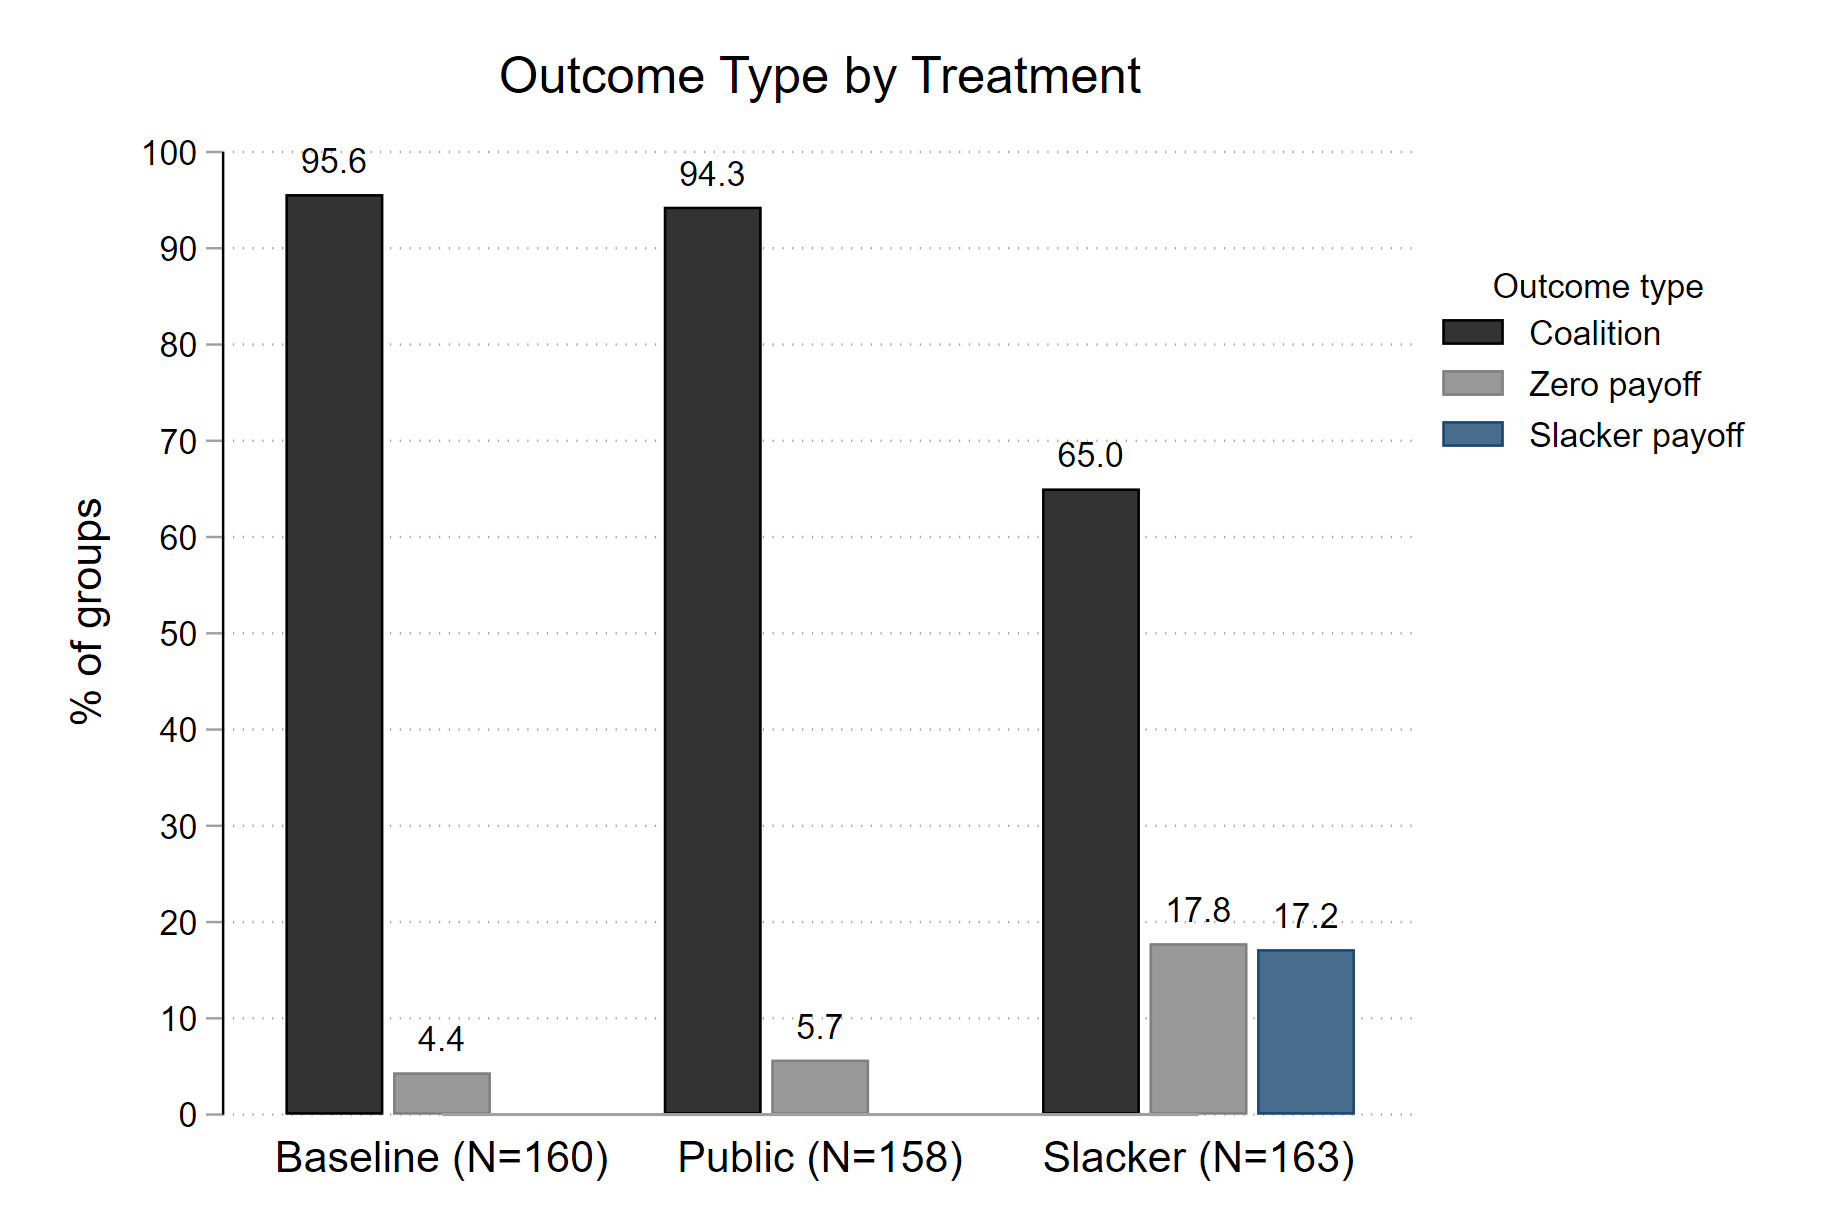
\includegraphics[width=\linewidth]{pic/Outcomes.png}
            \label{fig:outcome}
        \end{figure}
    \end{column}
\end{columns}

\end{frame}
\begin{frame}{Support NoOne}

\begin{columns}[c]
    \begin{column}{0.30\textwidth}
        \begin{itemize}
        \small
            \item Support no one Fisher's exact
            \begin{itemize}
            \small
                \item Baseline vs Public $p=0.000$
                \item Baseline vs Slacker $p=0.000$
            \end{itemize}
        \end{itemize}
    \end{column}

    \begin{column}{0.70\textwidth}
        \begin{figure}
            \centering
            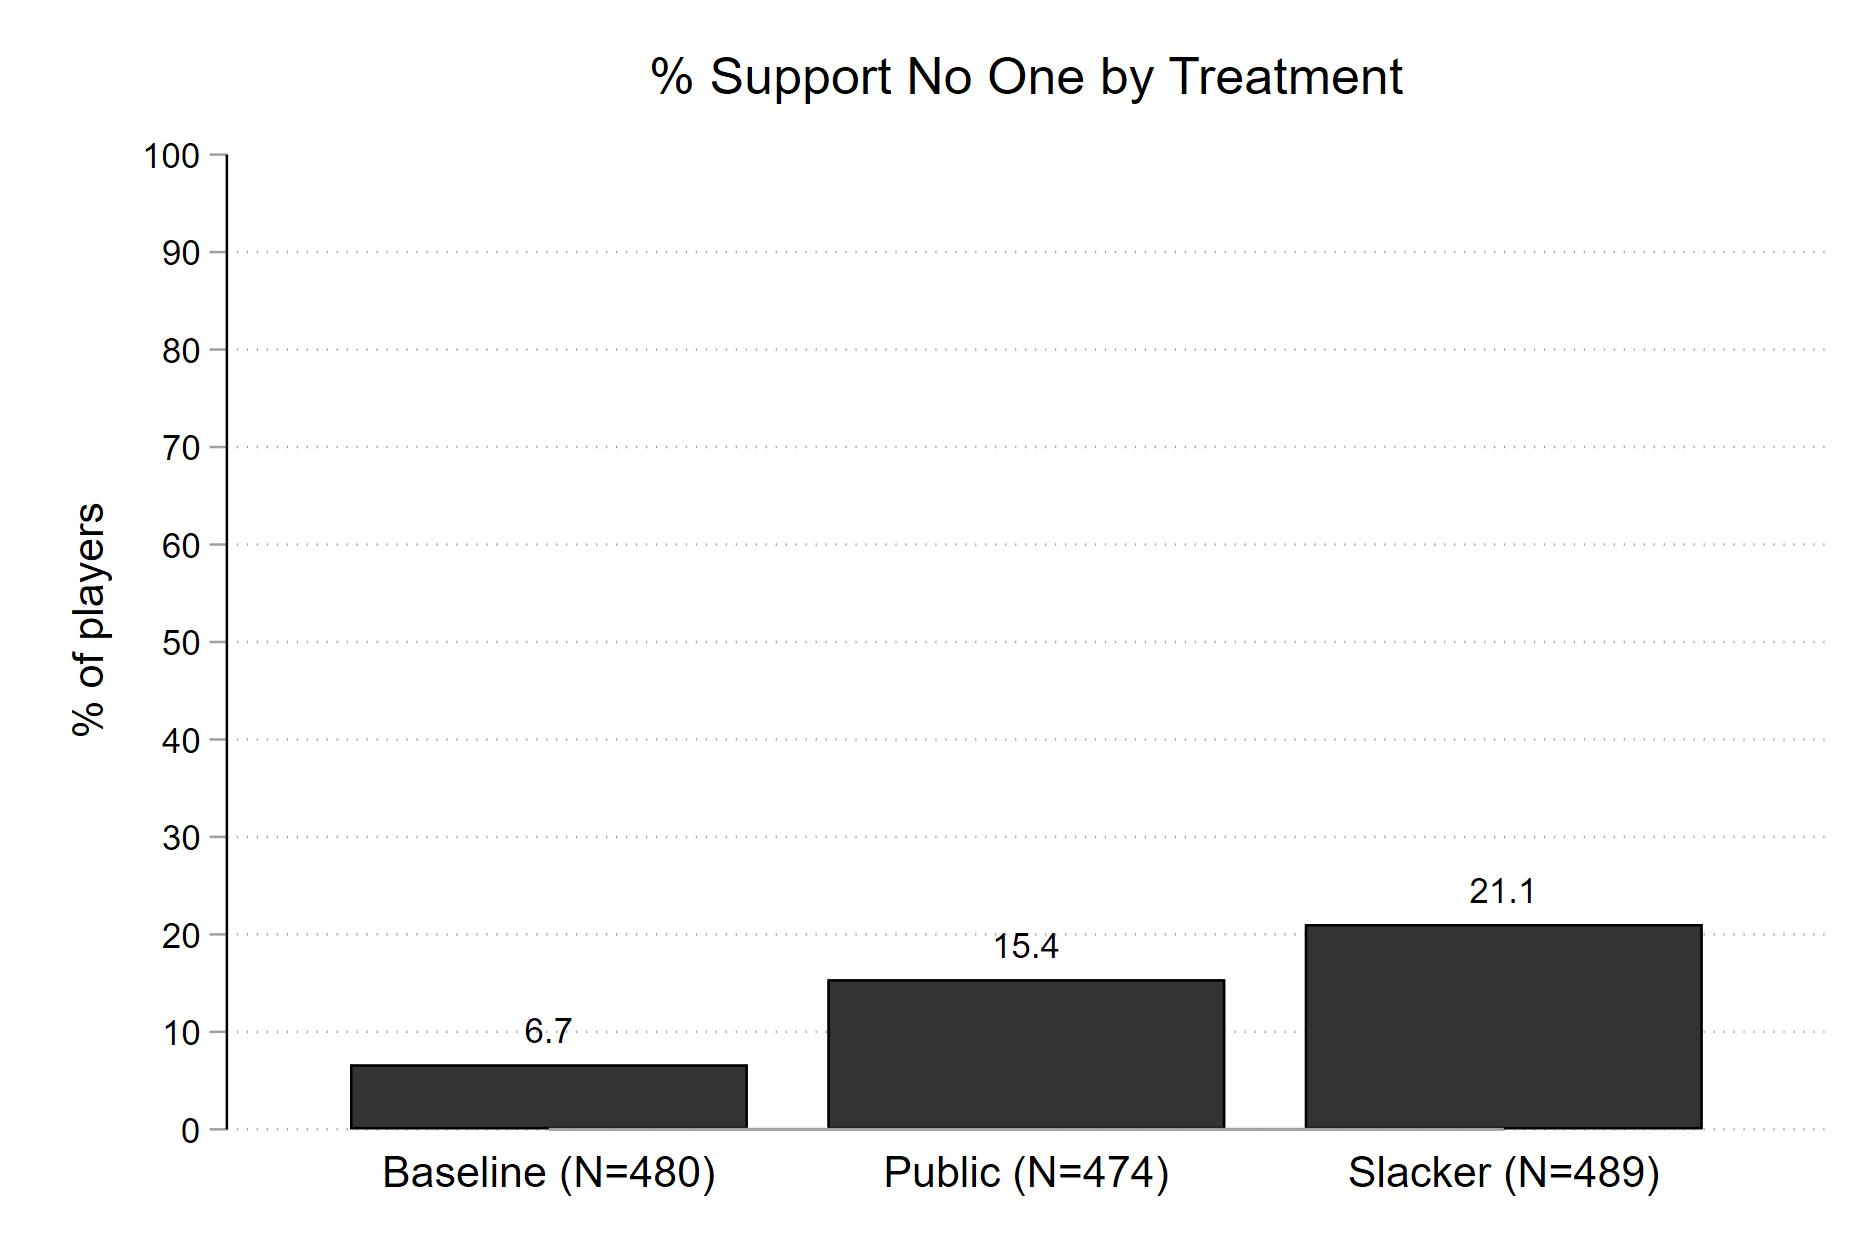
\includegraphics[width=\linewidth]{pic/Support_NoOne.png}
            \label{fig:Support_NoOne}
        \end{figure}
    \end{column}
\end{columns}

\end{frame}
\begin{frame}{Signal}

\begin{columns}[c]
    \begin{column}{0.30\textwidth}
        \begin{itemize}
        \small
            \item Honest Fisher's exact
            \begin{itemize}
            \small
                \item Baseline vs Public $p=0.000$
                \item Baseline vs Slacker $p=0.000$
            \end{itemize}
            \item Deceptive
            \begin{itemize}
            \small
                \item Baseline vs Public $p=0.000$
                \item Baseline vs Slacker $p=0.093$
            \end{itemize}
        \end{itemize}
    \end{column}

    \begin{column}{0.70\textwidth}
        \begin{figure}
            \centering
            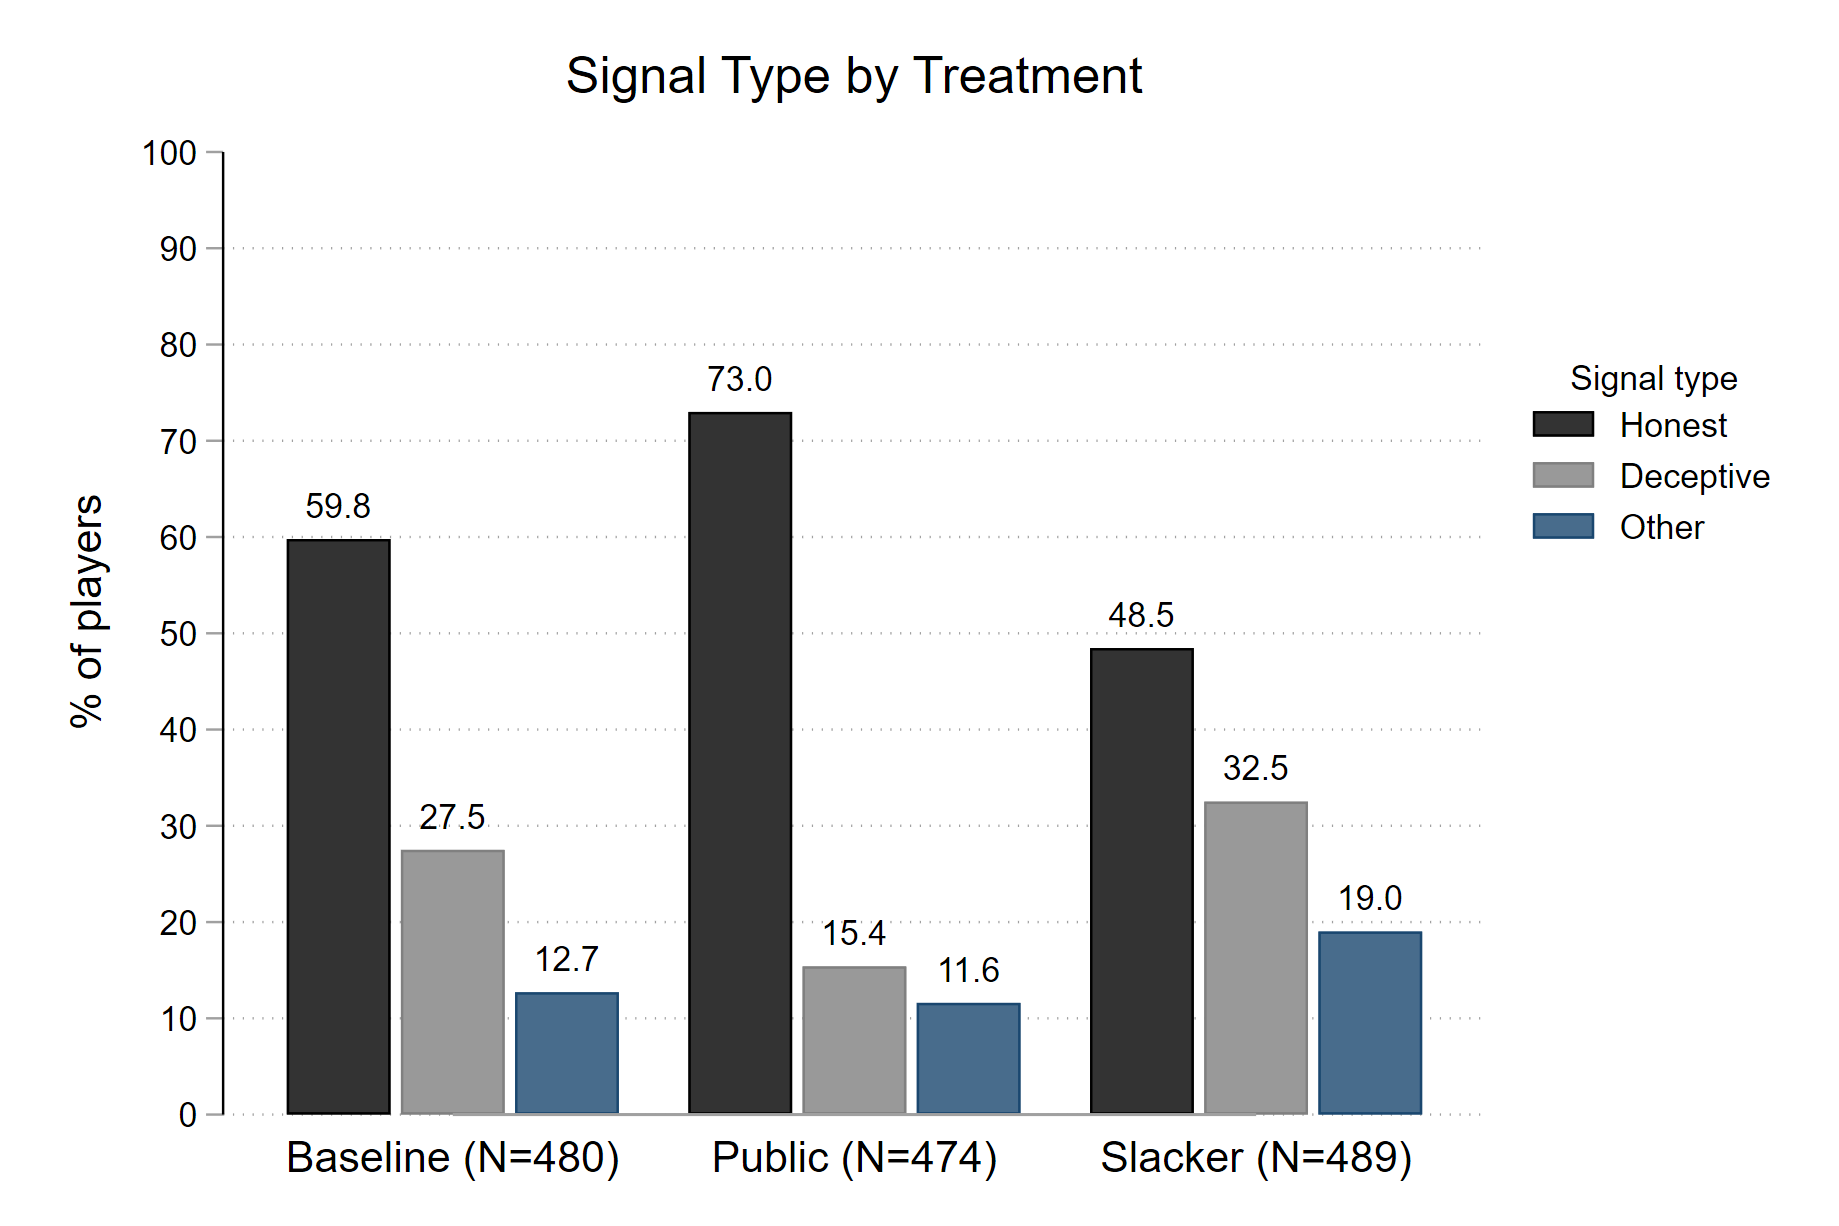
\includegraphics[width=\linewidth]{pic/Signal.png}
            \label{fig:Signal}
        \end{figure}
    \end{column}
\end{columns}

\end{frame}
\begin{frame}{Consistency}

\begin{columns}[c]
    \begin{column}{0.30\textwidth}
        \begin{itemize}
        \small
            \item Fisher's exact
            \begin{itemize}
            \small
                \item Baseline vs Public $p=0.022$
                \item Baseline vs Slacker $p=0.000$
            \end{itemize}            
        \end{itemize}
    \end{column}

    \begin{column}{0.70\textwidth}
        \begin{figure}
            \centering
            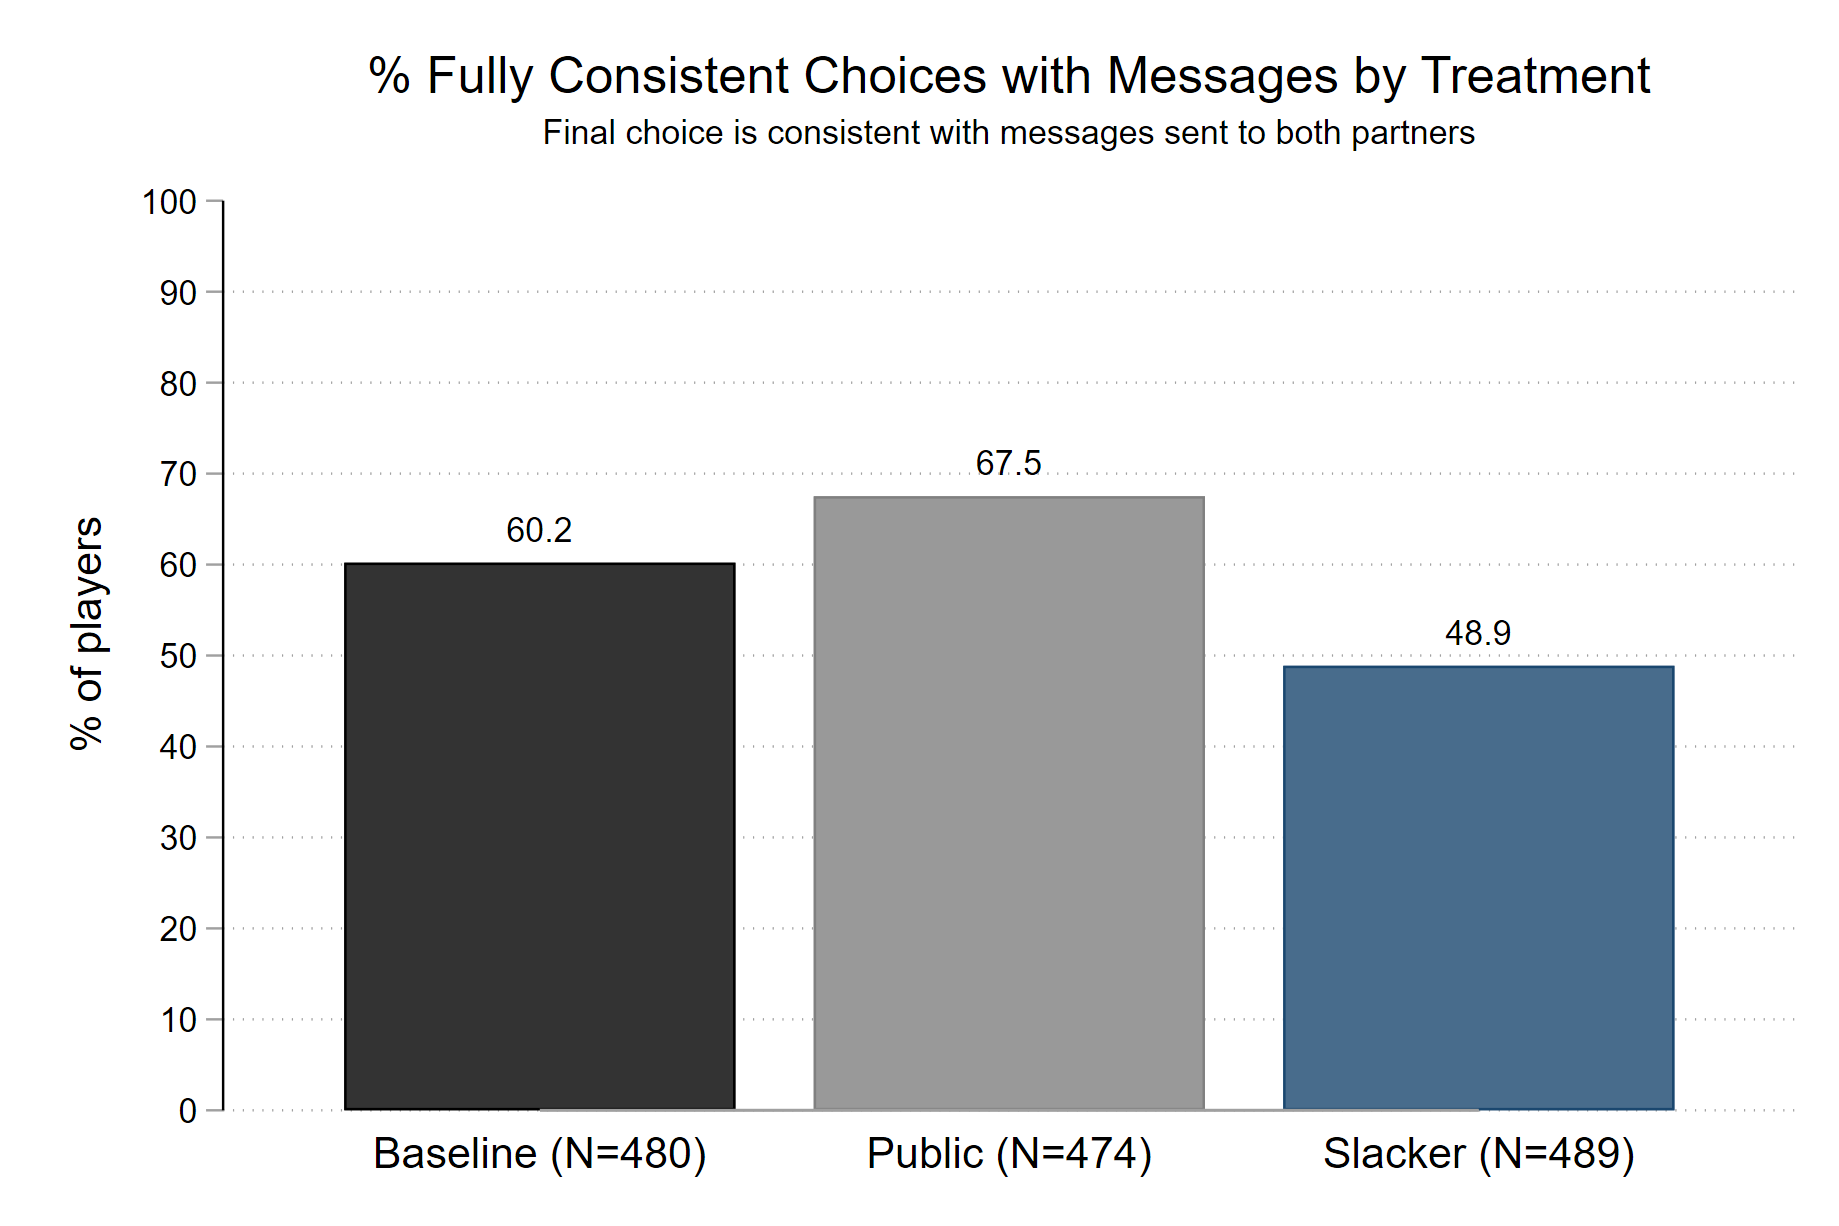
\includegraphics[width=\linewidth]{pic/SignalChoice_consistency.png}
            \label{fig:consistency}
        \end{figure}
    \end{column}
\end{columns}

\end{frame}

\begin{frame}{Strategic Deception}

\begin{columns}[c]
    \begin{column}{0.30\textwidth}
        \begin{itemize}
        \small
            \item Fisher's exact
            \begin{itemize}
            \small
                \item Baseline vs Public $p=0.115$
                \item Baseline vs Slacker $p=0.000$
            \end{itemize}            
        \end{itemize}
    \end{column}

    \begin{column}{0.70\textwidth}
        \begin{figure}
            \centering
            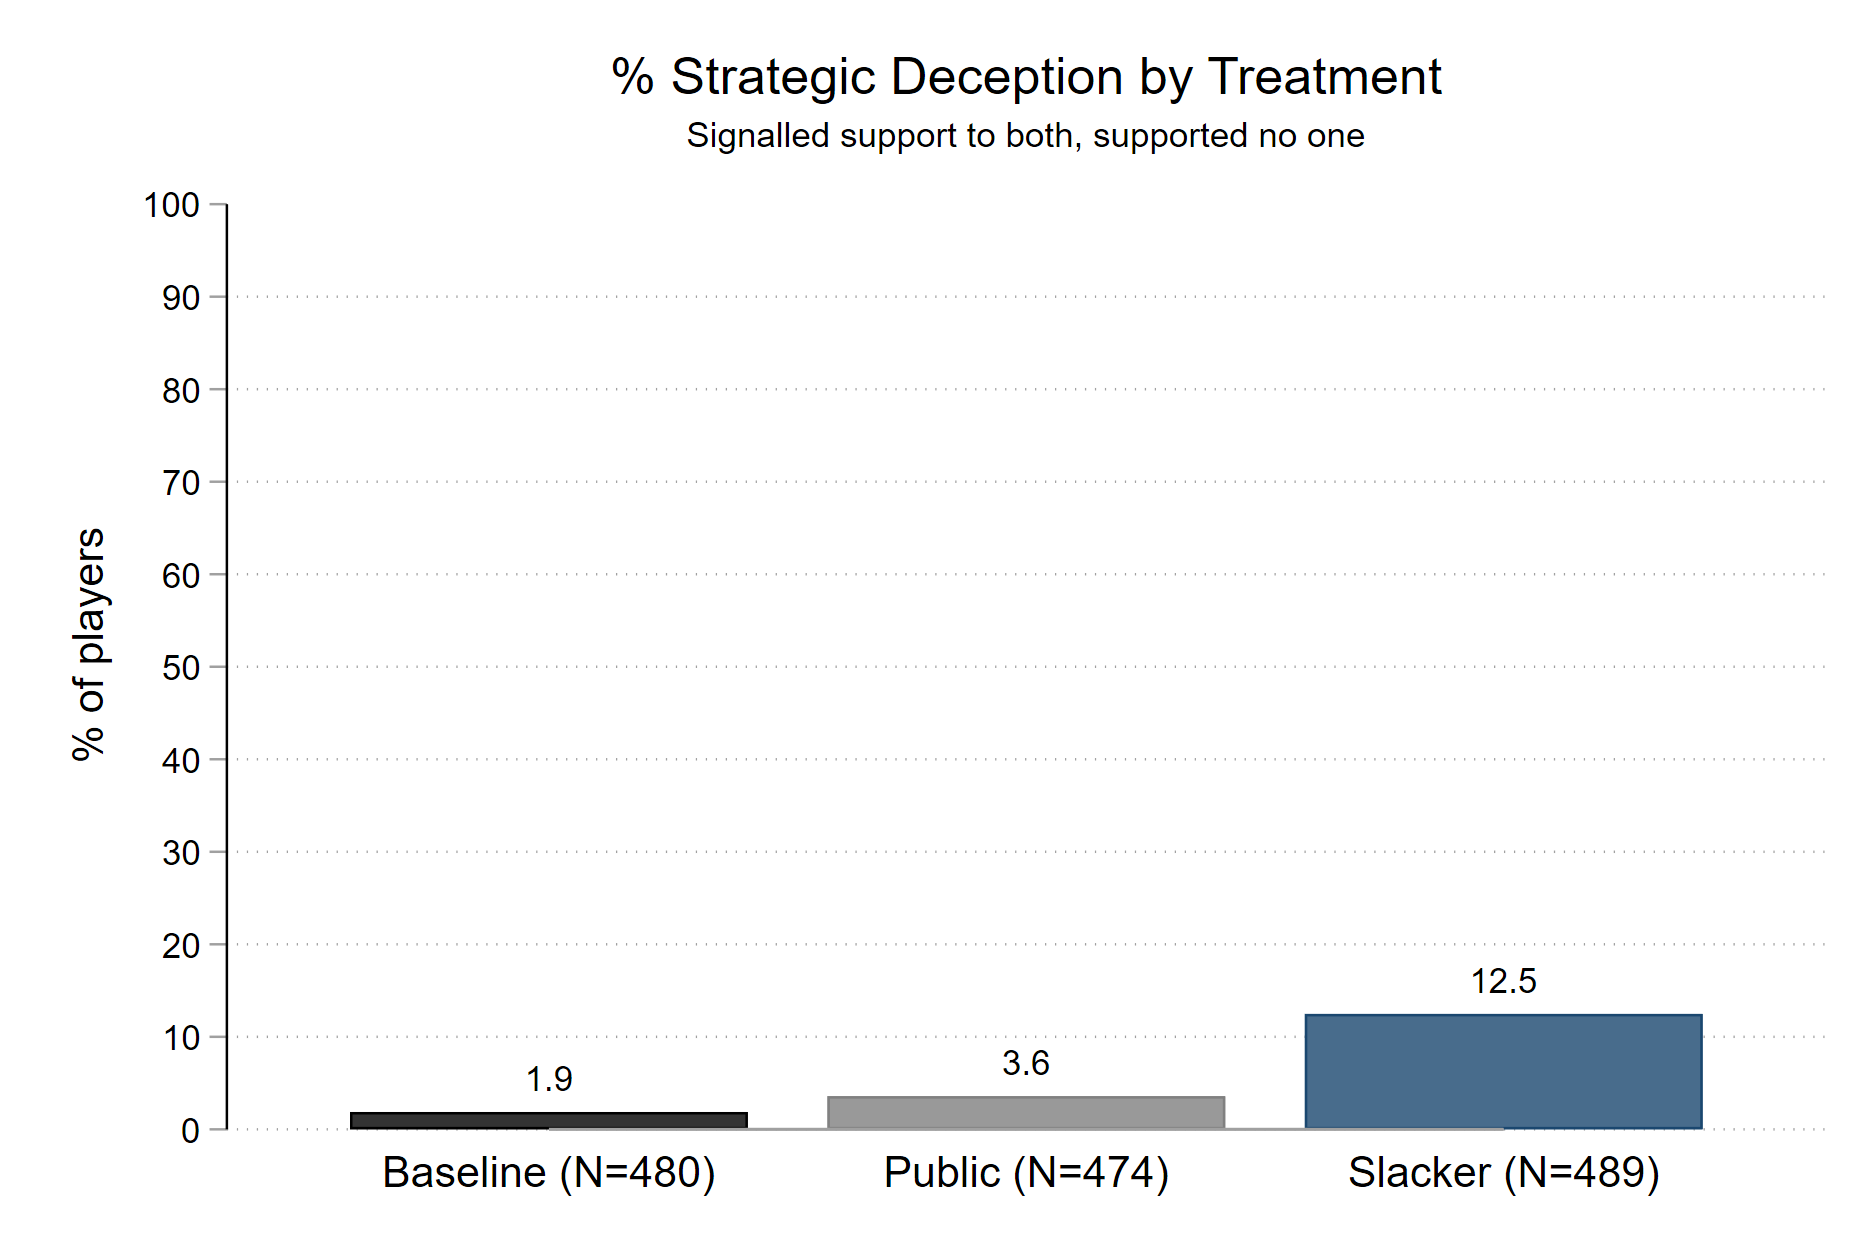
\includegraphics[width=\linewidth]{pic/Strategic_deception.png}
            \label{fig:StrategicDeception}
        \end{figure}
    \end{column}
\end{columns}

\end{frame}
\section{Text Analysis}
\begin{frame}{Messages}\justifying
\small
\textbf{Private}
\textit{Purple \rightarrow Yellow: "You're the first person to message me back so I think we should work together";
Purple \rightarrow Orange: "You were the first person to message me back so I think we should work together";
Yellow \rightarrow Purple: "Sounds good to me. That means at least we will both get money!"
Purple \rightarrow Yellow: "Yes exactly. Or else we're winding up with nothing"}


\textbf{Public}

\textit{Purple: "interesting dilemma, how to choose who to support... honestly was about to flip a coin... ah fate you fickle mistress"; Orange: "do you want to be heads or tails?"; Purple: "im going to start singing sinatra lol... tails please"; Yellow: "heads! do it!"
Purple: "may the odds be ever in your favor yellow, i salute you"; Orange: "it came up tails... should I do the best 2 out of 3?"; Yellow: "yeah!"
Orange: "it came up heads 2 times!"}

\textbf{Slacker}

Purple \rightarrow Orange: "Are you looking to make some easy money today for fun? Yeah, let's keep it simple. We vote for each other and make \$3."; Orange \rightarrow Purple: "I sure am! Perfect!"; Purple \rightarrow Yellow: "Are you looking to make some easy money today for fun? Cool, let's just vote for each other and make \$3."; Yellow \rightarrow Purple: "Sounds great to me! Awesome!"; Purple \rightarrow Both: "Great! / Awesome!"
\end{frame}


\begin{frame}{Messages}\justifying
\begin{figure}
    \centering
    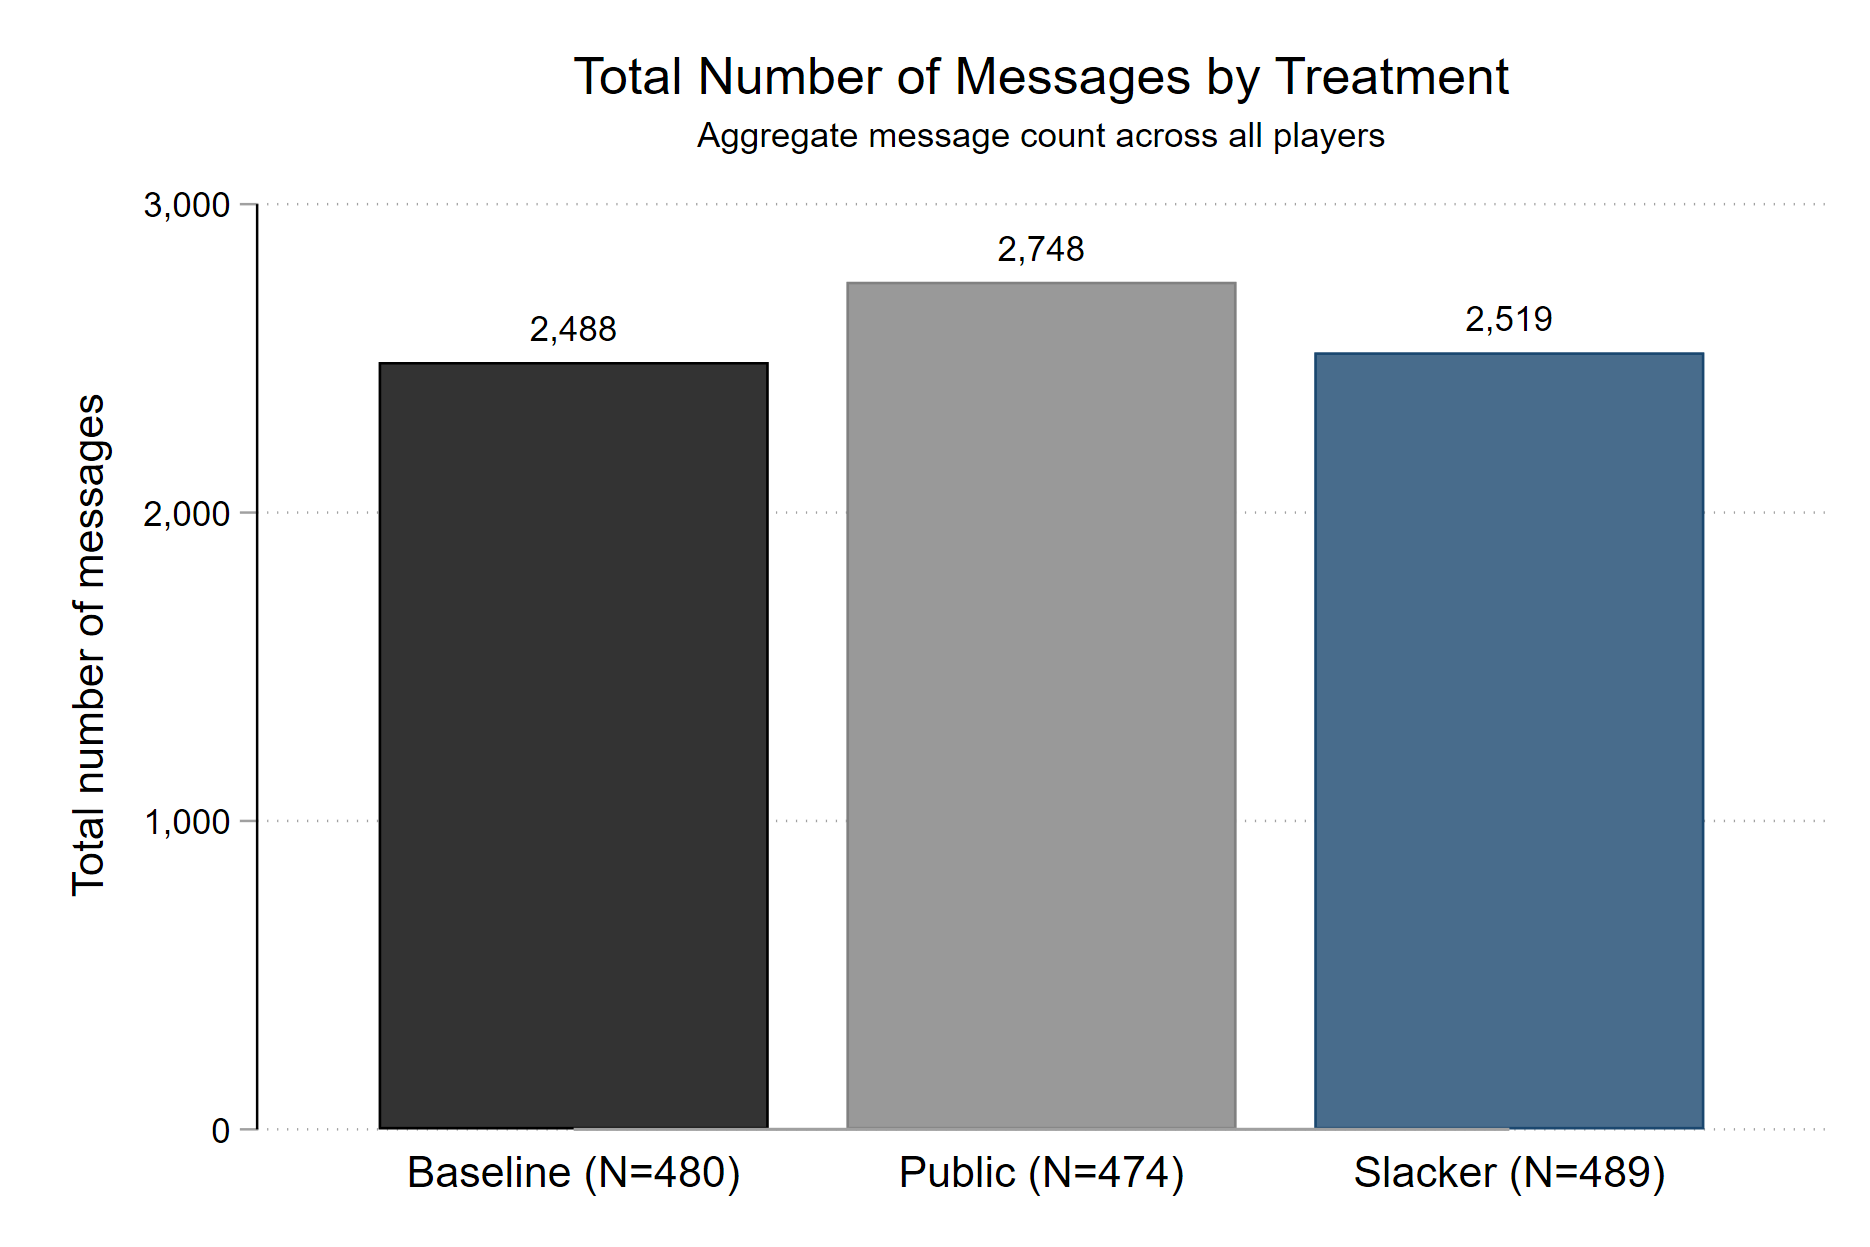
\includegraphics[width=0.70\linewidth]{pic/Nmessages.png}
    \label{fig:Nmessages}
\end{figure}
\end{frame}

\begin{frame}{Text Analysis}\justifying
\small
TopicGPT(\citealt{pham2024topicgpt, fieberg2025predicting}), and prompting LLM, we extract: \textit{volume, emotional tone, sentiment, analytical thinking Clout, Authenticity}\\
\textbf{Coalition Proposal}:
\begin{itemize}
    \item Hello, I propose we support each other to earn \$3;
    \item I'm the purple participant. I'm willing to form an alliance. I will support you in order to do the same if you support me. Sounds like a plan!
\end{itemize}
\textbf{Commitment}:
\begin{itemize}
    \item Doing good, let's make this real simple and lock it down right now. I choose you and you choose me, done deal;
    \item Do you want to be partners in this round? Okay, I'm 100\% going to choose you. Pinky promise lol
\end{itemize}
\textbf{Payoff Reasoning}:
\begin{itemize}
    \item I wish there were a way to have everyone split 6 three ways, but since there isn't and someone has to be left out, you seem reasonable. Let's split;
    \item I don't think there's a fair way to do this right, like one person has to be left out. Yeah, I'm gonna sacrifice myself and take the hit, vote for the other.
\end{itemize}
 \vspace{0.3\baselineskip} 
\end{frame}
\section{What is Persuasive?}
\begin{frame}{Determinants of Persuasion: Logistic Regressions (1--6)}
    \begin{figure}
        \centering
        \vspace*{-0.4cm}
        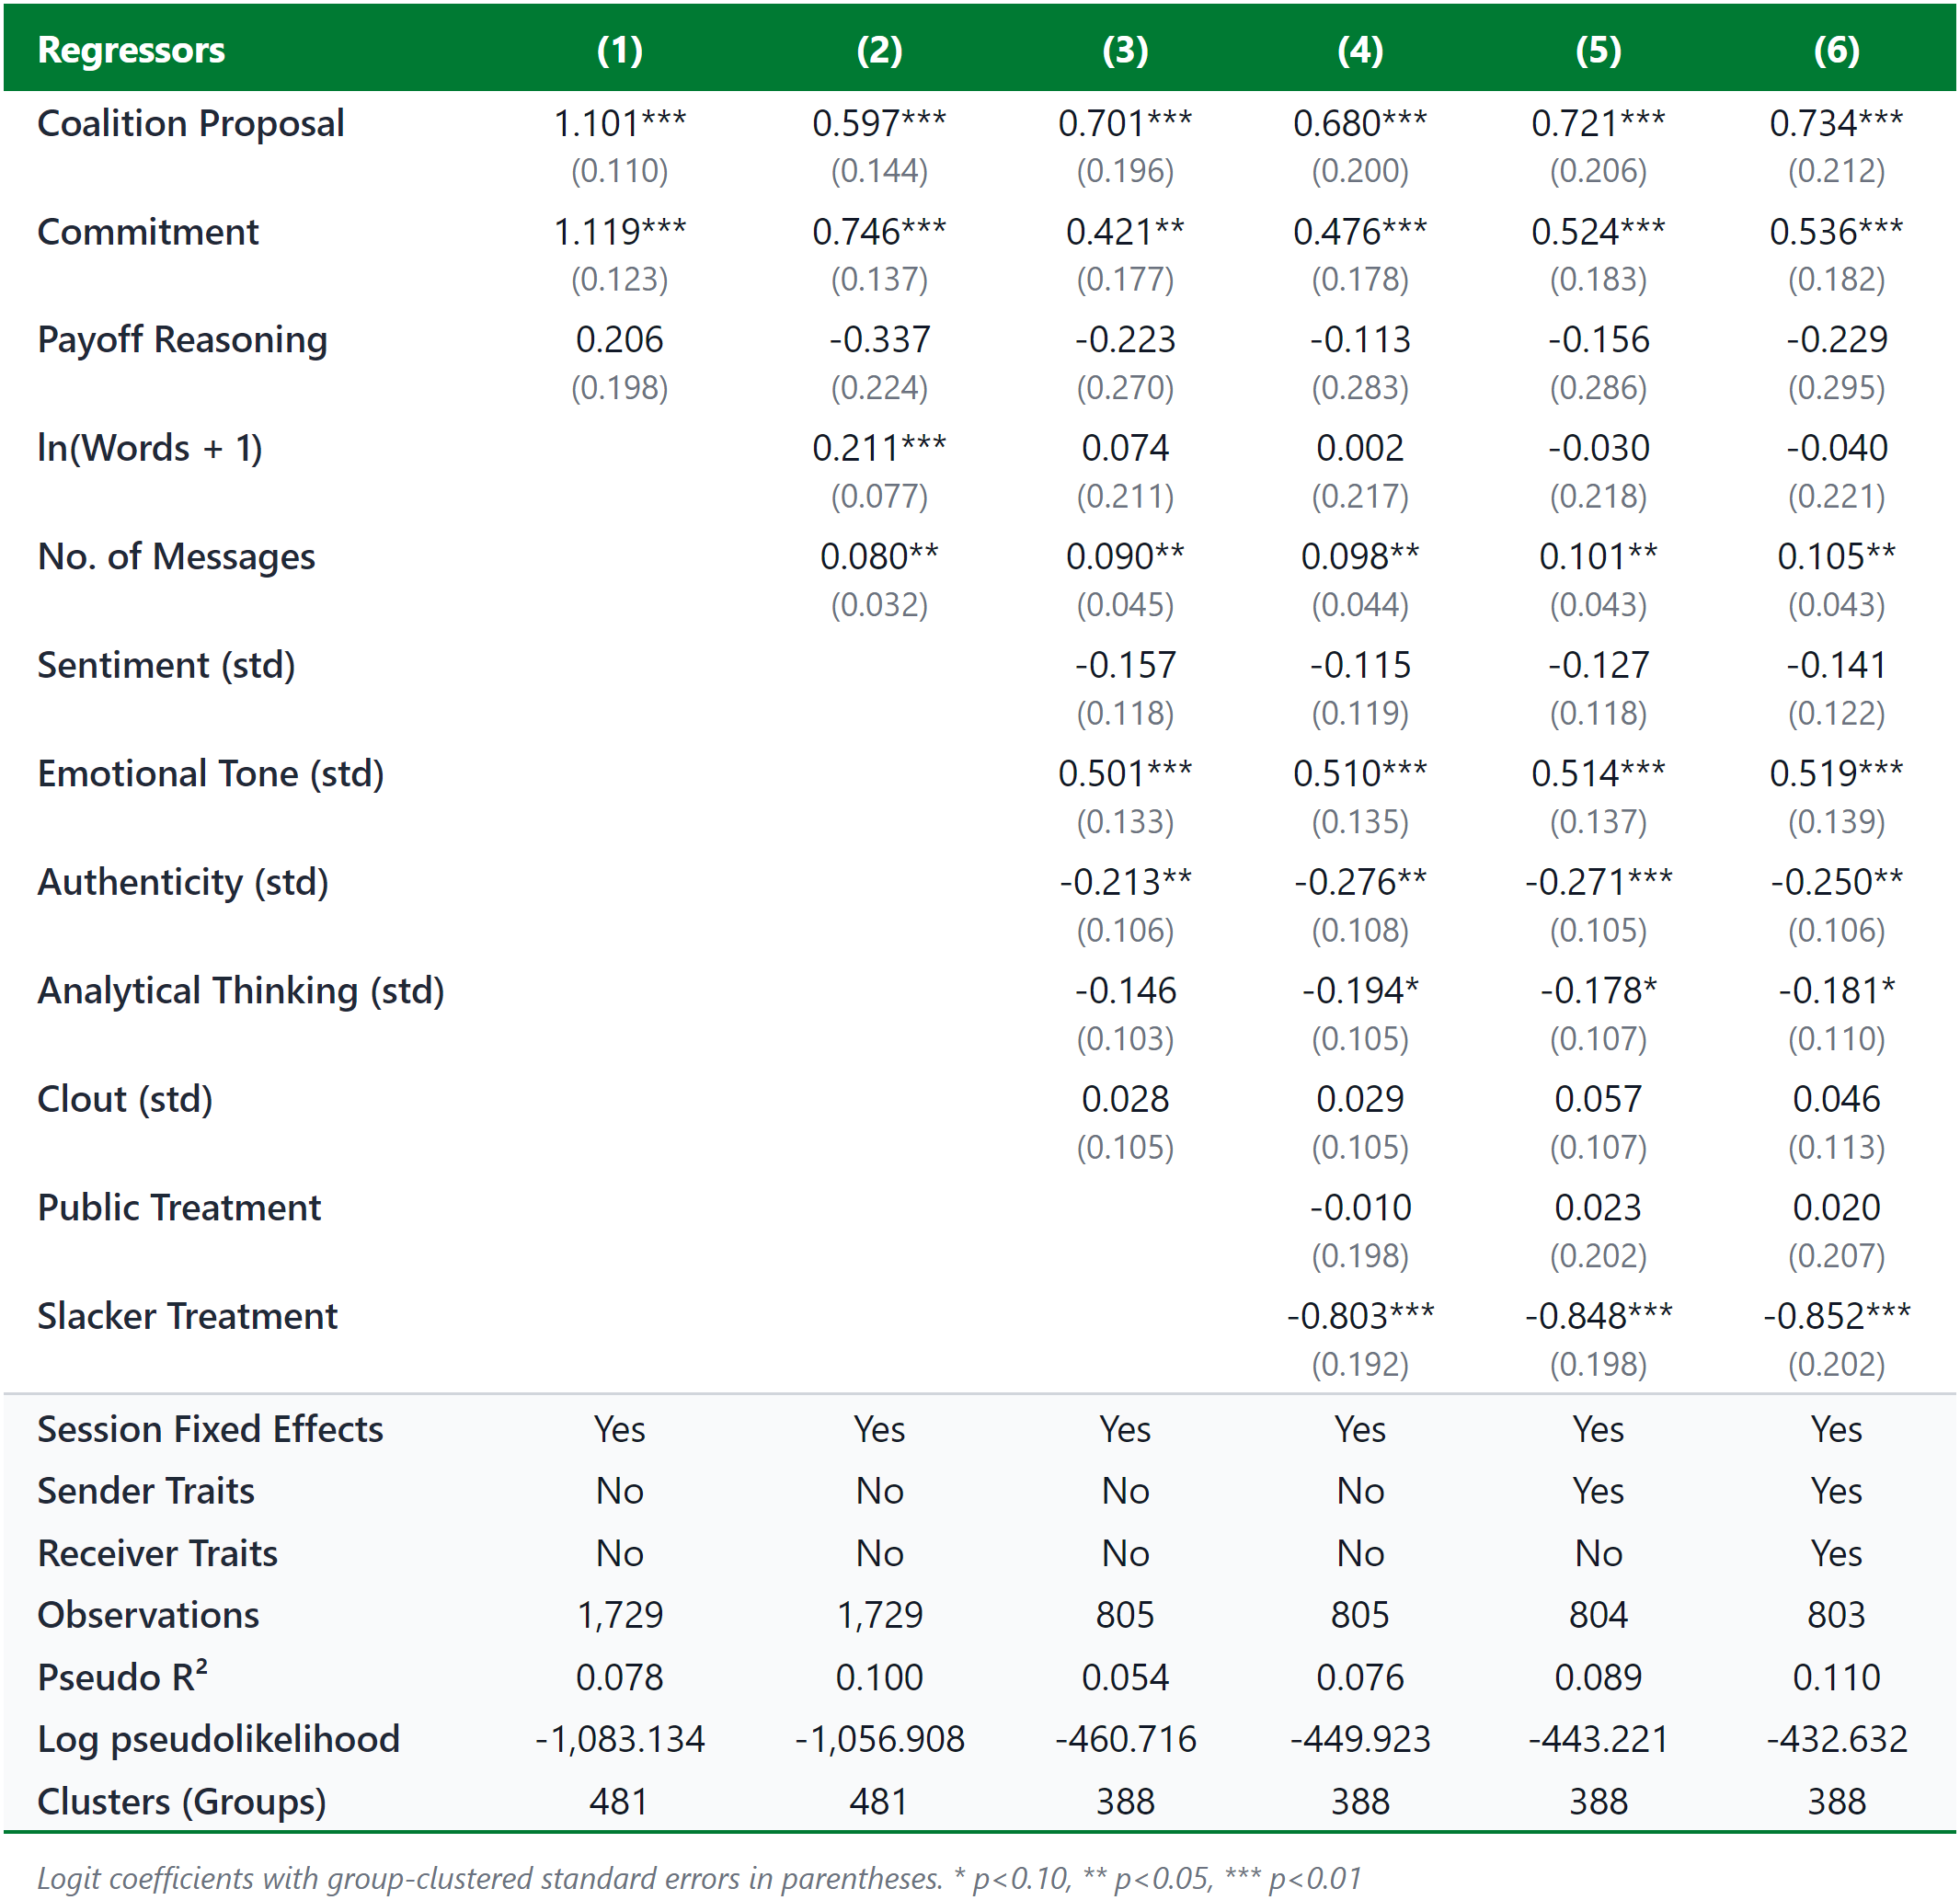
\includegraphics[height=0.82\textheight]{pic/tab_persuasion_logit_6models.png}
    \end{figure}
\end{frame}

\begin{frame}{Determinants of Persuasion: Average Marginal Effects ($dy/dx$)}
    \begin{figure}
        \centering
        \vspace*{-0.4cm}
        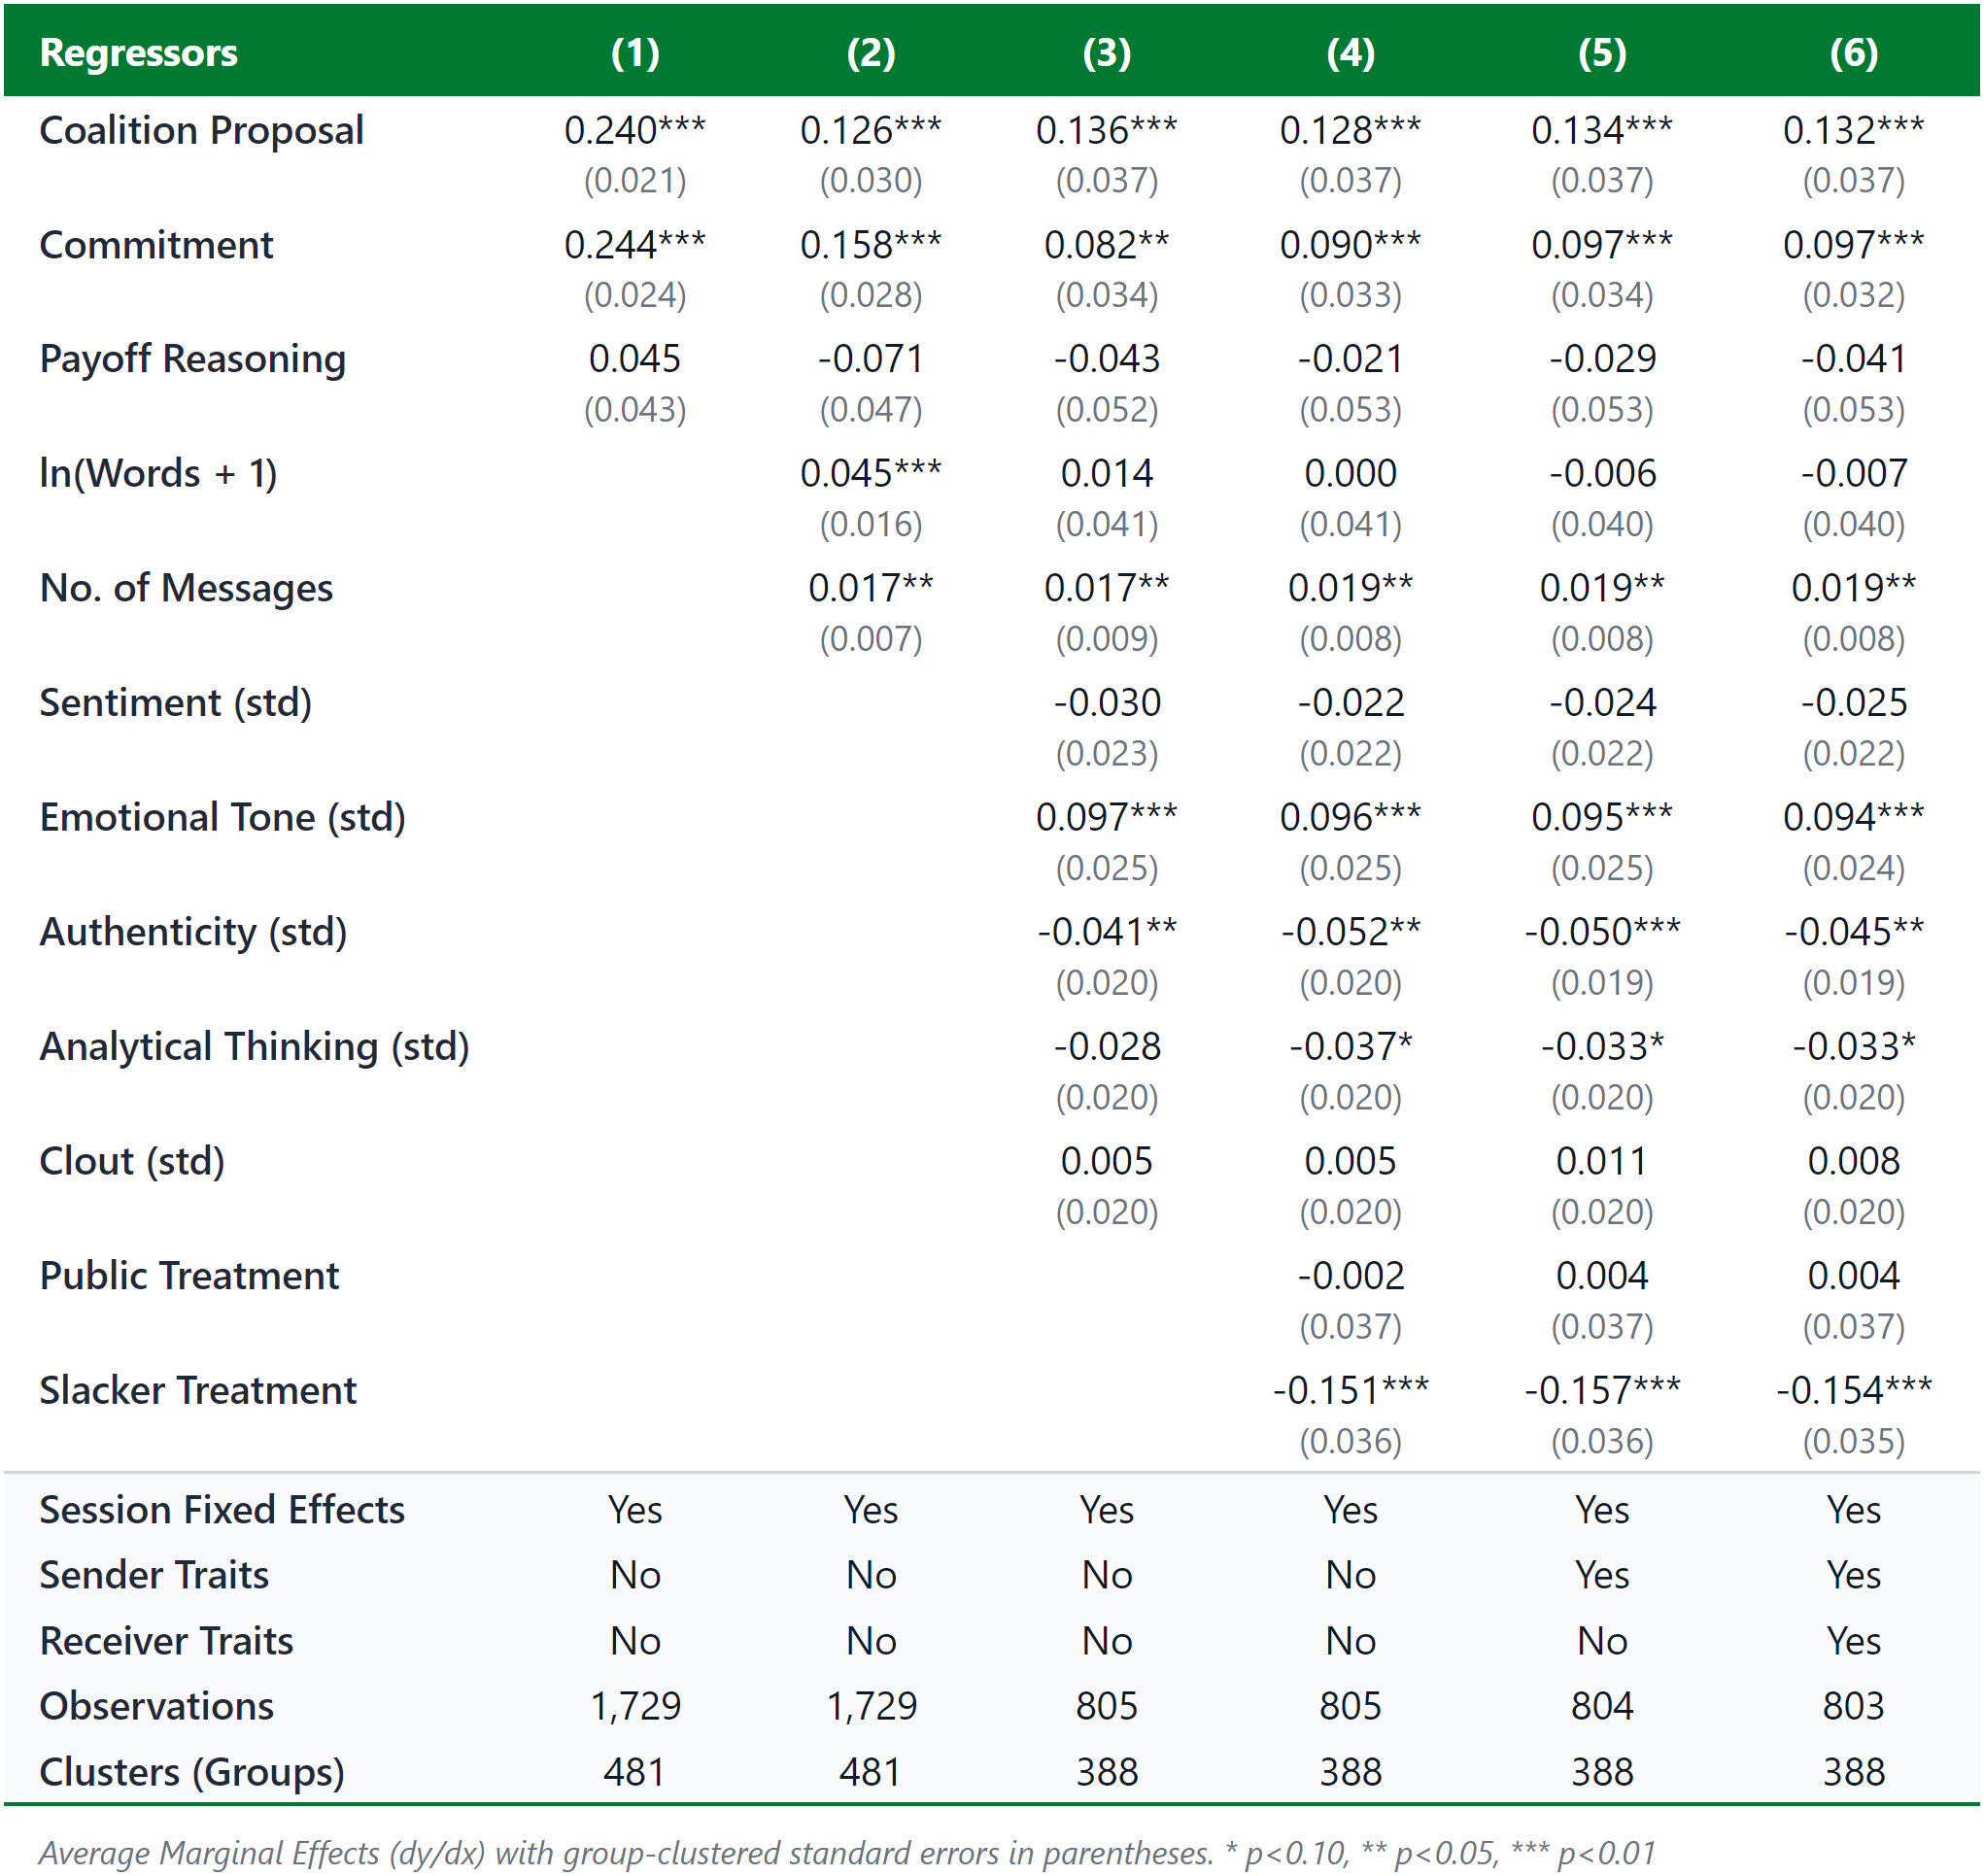
\includegraphics[height=0.82\textheight]{pic/tab_persuasion_logit_ame_6models.png}
    \end{figure}
\end{frame}
\section{Conclusion}
\begin{frame}
    \begin{center}
        {\Huge\calligra Thank You}
    \end{center}
\end{frame}

\section{References}

\begin{frame}[allowframebreaks]{References}
    \bibliography{ref}
    \bibliographystyle{apalike}
    \nocite{*} 
\end{frame}

\end{document}